\documentclass[pdf]{beamer}
\usepackage[latin1]{inputenc}
\usepackage{multirow}
\usetheme{Warsaw} %Warsaw
\usecolortheme{beaver}

\begin{document}

\title[Quality Assurance and Preprocessing]{DNA Microarrays\\Quality Assurance and Preprocessing\\}
\subtitle{BCB 504: Applied Bioinformatics\\}
\author[Matt Settles]{Matt Settles}
\institute{University of Idaho\\ Bioinformatics and Computational Biology Program}
\date{\today}


%% Title page
\begin{frame}[plain]
  \titlepage
\end{frame}


%% Outline
\begin{frame}[plain] 
  \frametitle{Outline}
  \tableofcontents
\end{frame}

\section{Raw Data}
\begin{frame} 
  \frametitle{Components of Raw Data}
  \begin{itemize}
    \item Quantified intensities for each microarray probe (spot), usually identified by X,Y coordinate
    \begin{description}
      \item[Affymetrix] Binary CEL files
      \item[Nimblegen] plain text pair or xys files
    \end{description}
    \item Microarray description file, associates probes to probesets and genes
    \begin{description}
      \item[Affymetrix] CEL description files or CDF files (Bioconductor provides)
      \item[Nimblegen] Nimblegen description files or NDF Files (must create your own packages)
    \end{description}
  \end{itemize}
\end{frame}

%
\section{Quality Assurance}
\begin{frame}
  \frametitle{Quality Assurance}
  \begin{enumerate}
    \item Visual check of chip pseudo-images.
    \item Consistency across microarrays.
    \item Observed patterns meet expectations.
  \end{enumerate}
\end{frame}

\subsection{Chip Images}
\begin{frame}
  \frametitle{Pseudo-chip images}
  \begin{columns}[t] % contents are top vertically aligned
    \begin{column}[T]{5cm} % each column can also be its own environment
      \begin{itemize}
        \item Pseudo-chip images are created from the data themselves and not from the original scanned images
        \item Can be created from the raw intensities, log intensities, model fitting residuals and other
        \item Looking for large anomalies
      \end{itemize}
     \end{column}
     \begin{column}[T]{5cm} % alternative top-align that's better for graphics
        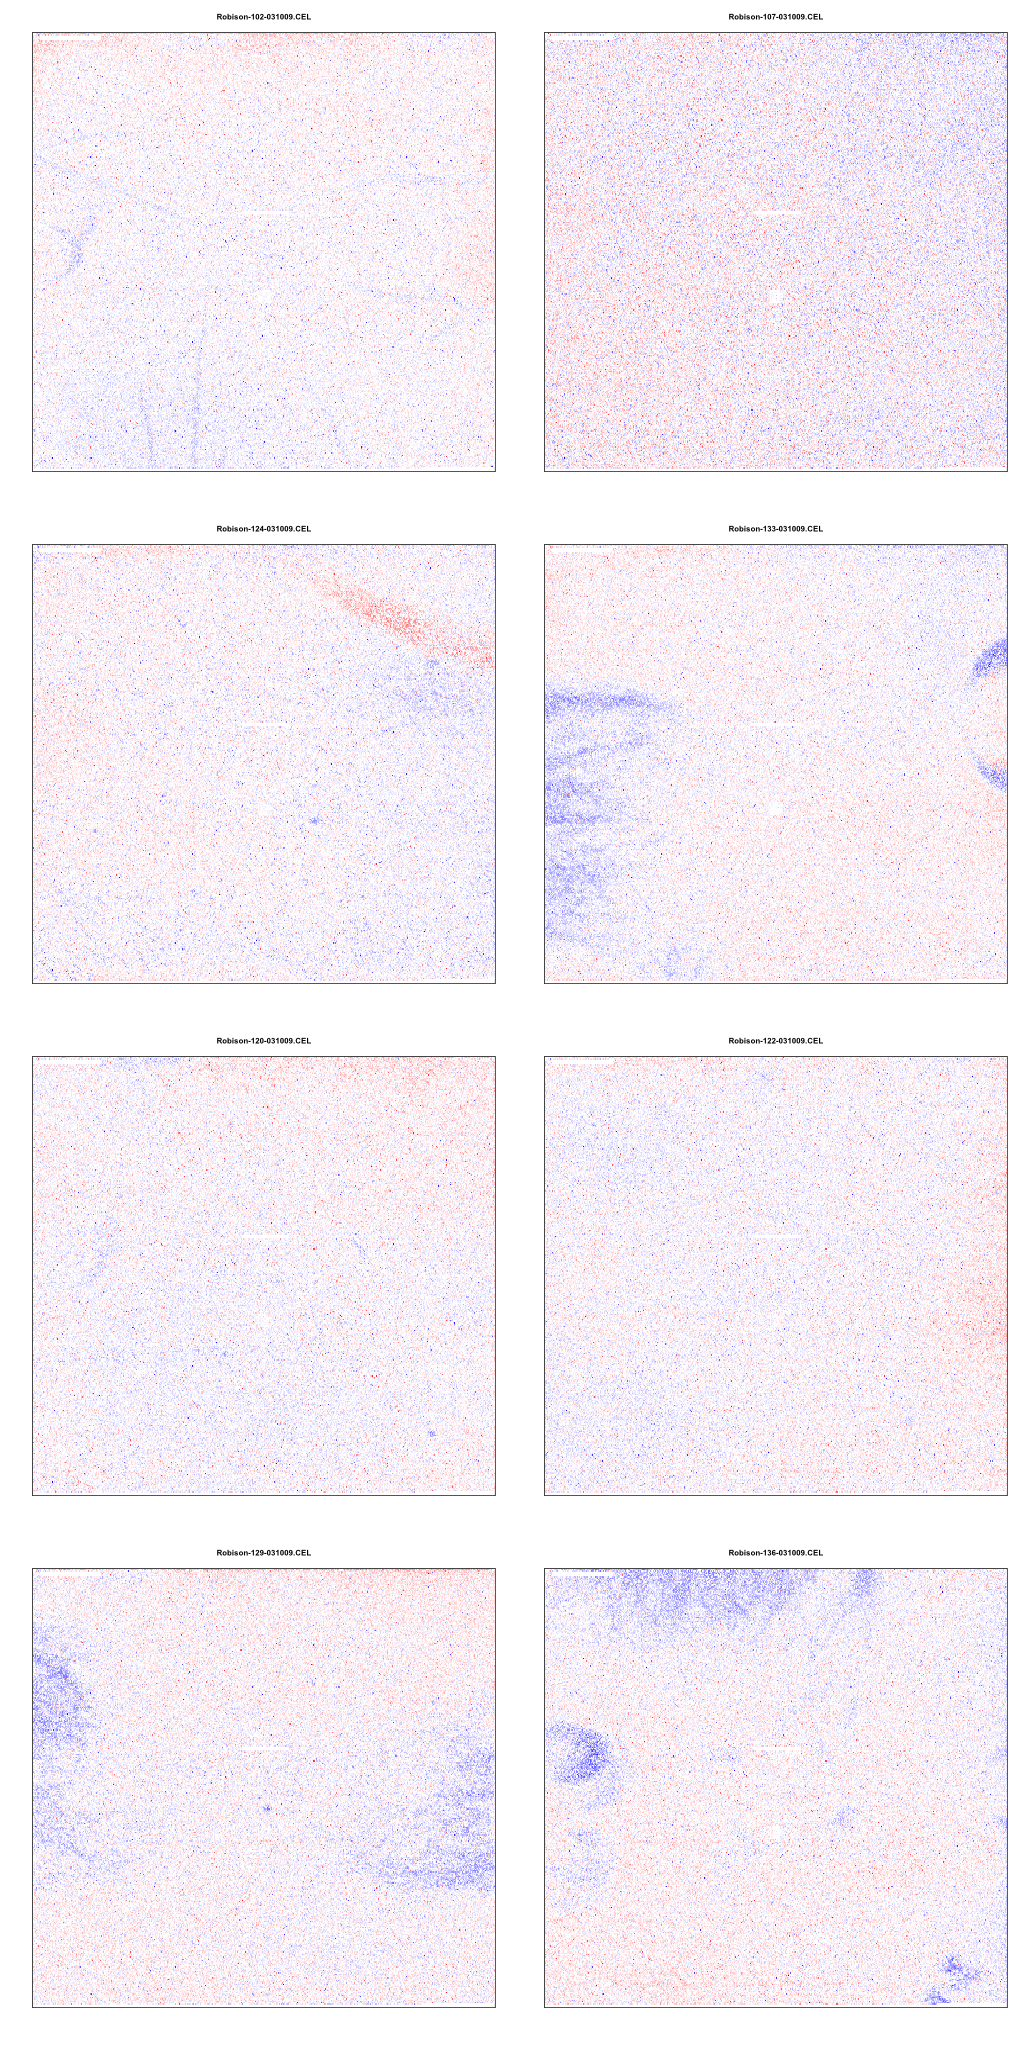
\includegraphics[scale=0.1]{figures/resid0.png} 
     \end{column}
  \end{columns}
\end{frame}

\subsection{Consistency}
\begin{frame}
  \frametitle{Consistency across microarrays}
  \begin{center}
  \centering 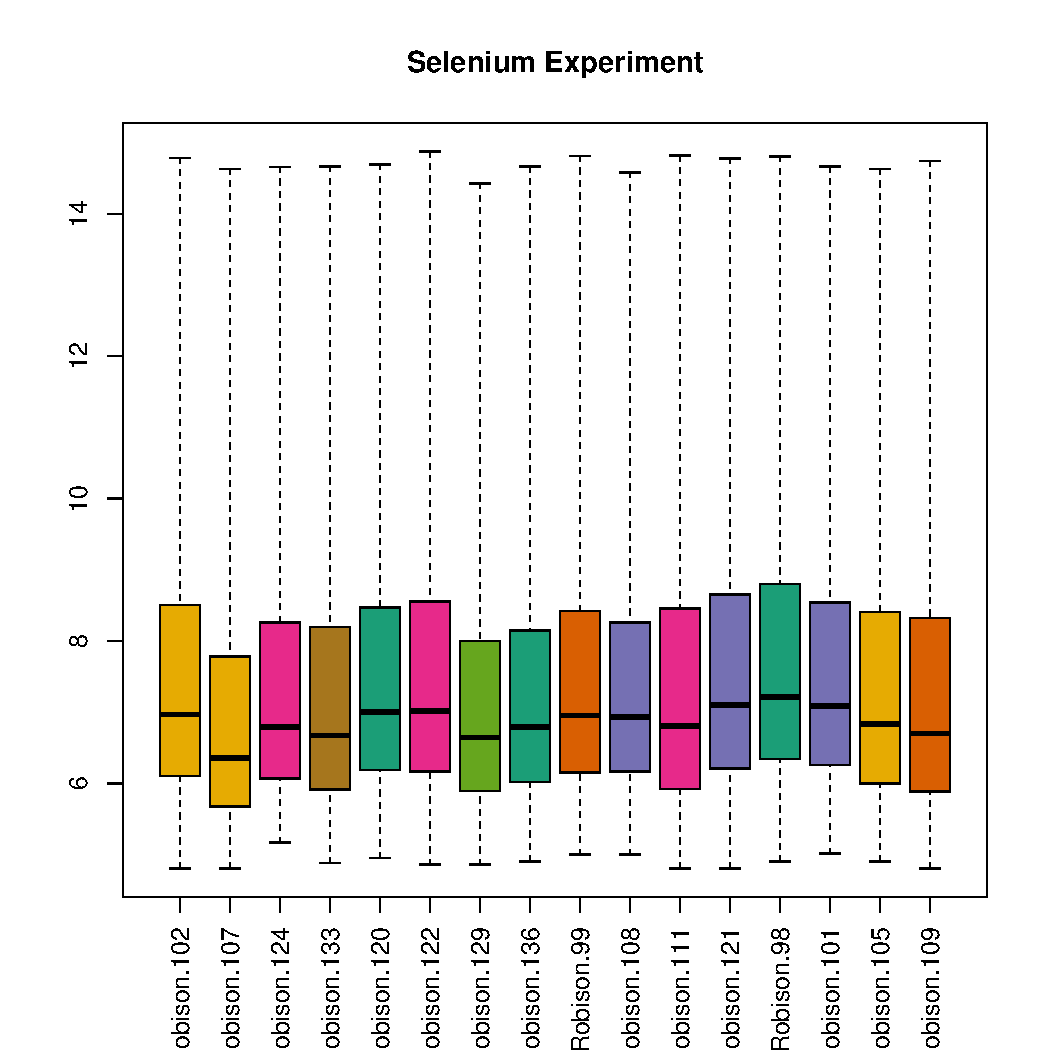
\includegraphics[scale=0.45]{figures/affybxp.pdf}
  \end{center}
\end{frame}

\begin{frame}
  \begin{center}
  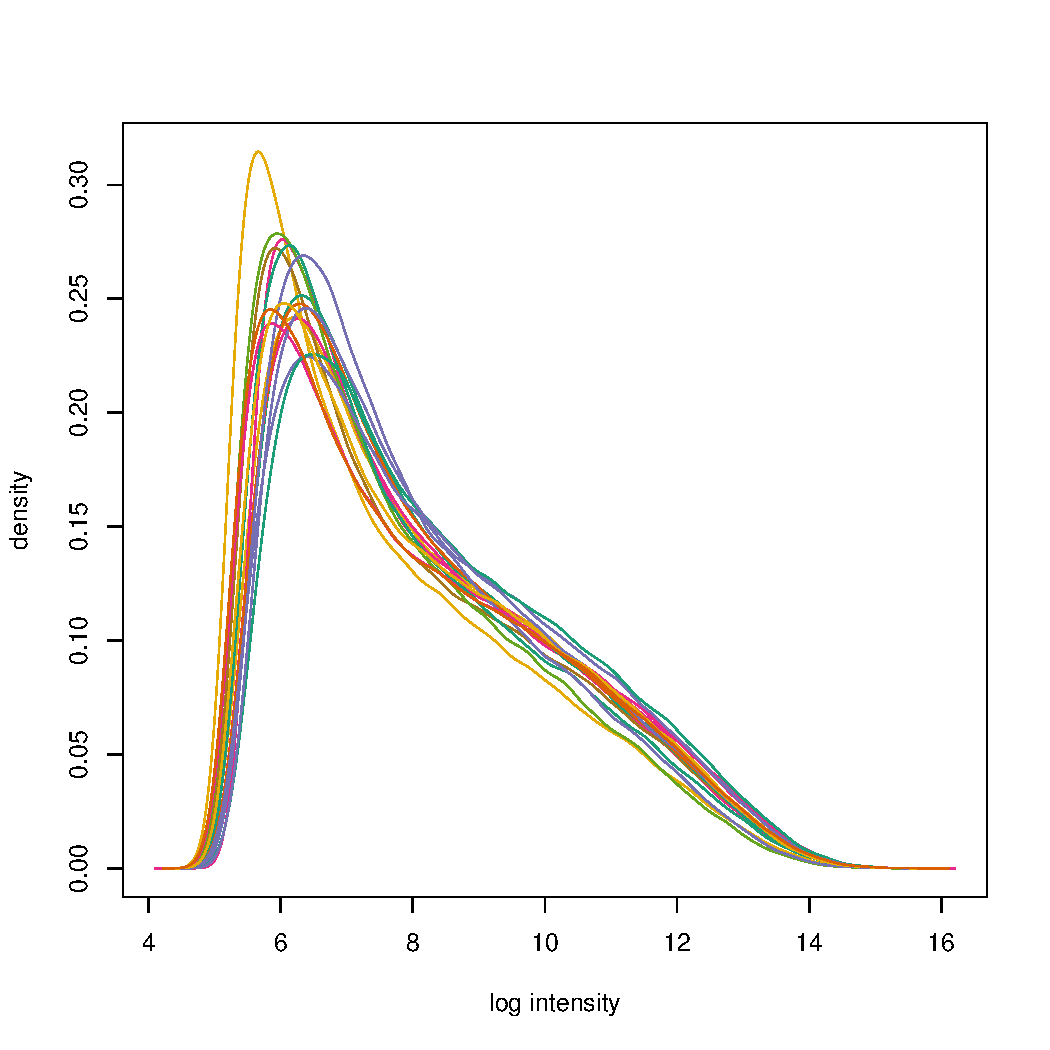
\includegraphics[scale=0.45]{figures/affyhist.pdf}  
  \end{center}
\end{frame}

\begin{frame}
  \begin{center}
  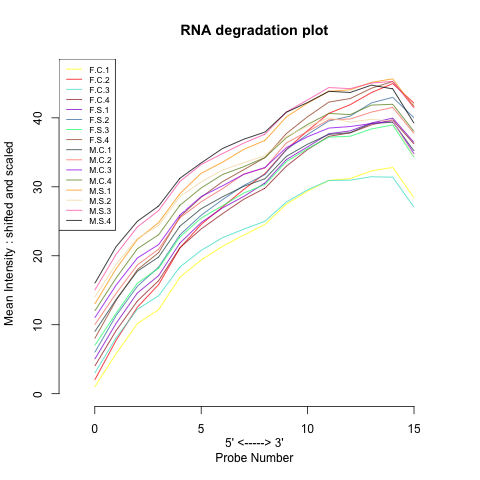
\includegraphics[scale=0.5]{figures/Figure2.png} 
  \end{center}
\end{frame}

\subsection{Expectations} 

\begin{frame}
  \frametitle{Expectations}  
  \begin{center}
  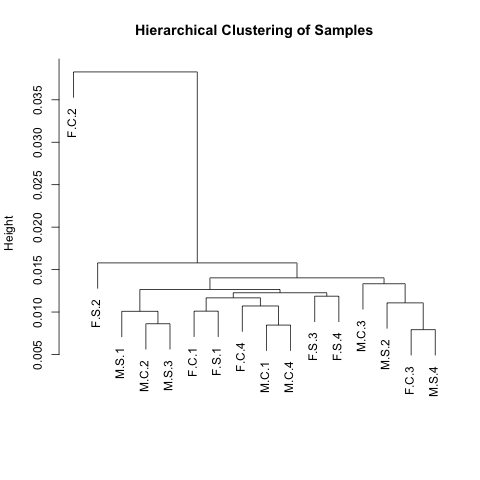
\includegraphics[scale=0.5]{figures/Figure3.png} 
  \end{center}
\end{frame}


\section{Preprocessing}
\begin{frame}
  \frametitle{Preprocessing}
  The goals of preprocessing Affymetrix microarray data are three fold:
  \begin{enumerate}
    \item To remove variation due to technical sources, while preserving variation from biological sources. 
    \item To normalize a set of microarrays in order to make them comparable.
    \item To produce summarized expression values for each probe set.
  \end{enumerate} 
\end{frame}

\begin{frame}
  \begin{description}
    \item[Background correction] Deviations from actual expression levels are introduced by many sources including scanner artifacts, non-specific binding (hybridization), RNA quality, reagents, etc.. All of which can be considered as background noise.
    \item[Probe level normalization] The role of normalization is to compensate for the technical effects, while preserving the effects due to the biology.
    \item[PM Correction] PM correction routines are designed to account for non-specific binding by use of the MM probes.
    \item[Probe set summarization] Probe set summarization produces a single value for a probe set that is the estimated expression level for the probe set (i.e. gene).
    \item[Probe set normalization] Same purpose as Probe level normalization but on the probe sets.
  \end{description}
\end{frame}

\subsection{Algorithms}
\begin{frame}
  \begin{tiny}
  \begin{center}
  \begin{table}
  \caption{Breakdown of the preprocessing steps for the MAS5, Plier, RMA, GCRMA, and dChip preprocessing pipelines.}
  \begin{tabular}{|l|c|c|c|c|c|}
  \hline
  & \textbf{MAS5} & \textbf{Plier} & \textbf{RMA} & \textbf{GCRMA} & \textbf{dChip} \\ \hline
  Background & weighted   & \multirow{2}{*}{none} & RMA  & GCRMA & \multirow{2}{*}{none} \\
  Correction &  average  &  & (global model) & (model based) &  \\ \hline
  Probe Level &  \multirow{2}{*}{none}   & quantile  &  quantile  &  quantile  & invariant  \\
  Normalization  & &  normalization &   normalization &   normalization &  set\\ \hline
    \multirow{2}{*}{PM Correction} & ideal & \multirow{2}{*}{none} & \multirow{2}{*}{none} & \multirow{2}{*}{none} & subtract MM \\ 
    &  mismatch    & & & & none \\ \hline
  Probe set & Tukey & \multirow{2}{*}{Plier} & median  & median  & \multirow{2}{*}{MBEI}\\  
  Summarization &  biweight   &  &  polish &  polish &  \\ \hline
  Probe set & mean & \multirow{2}{*}{none} & \multirow{2}{*}{none} & \multirow{2}{*}{none} & \multirow{2}{*}{none}\\ 
  Normalization & scaled &  &  &  & \\ \hline
  \end{tabular}
  \end{table}
  \end{center}
  \end{tiny}
\end{frame}
   
\subsection{QA preprocessing}
\begin{frame}
\begin{center}
  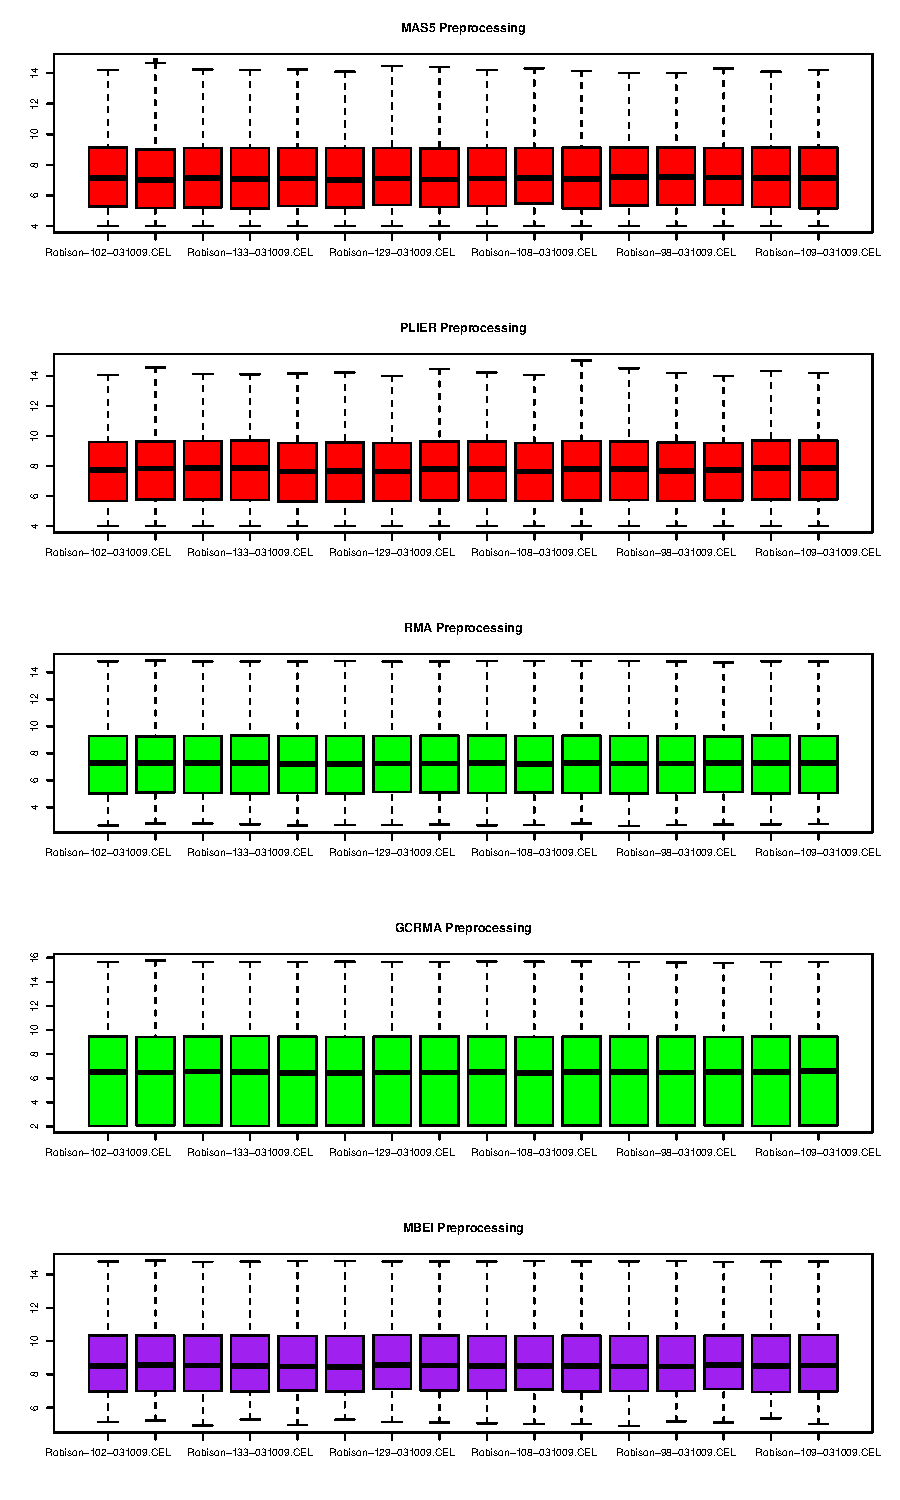
\includegraphics[scale=0.4]{figures/normboxplots.pdf} 
\end{center}
\end{frame}

\begin{frame}
\begin{center}
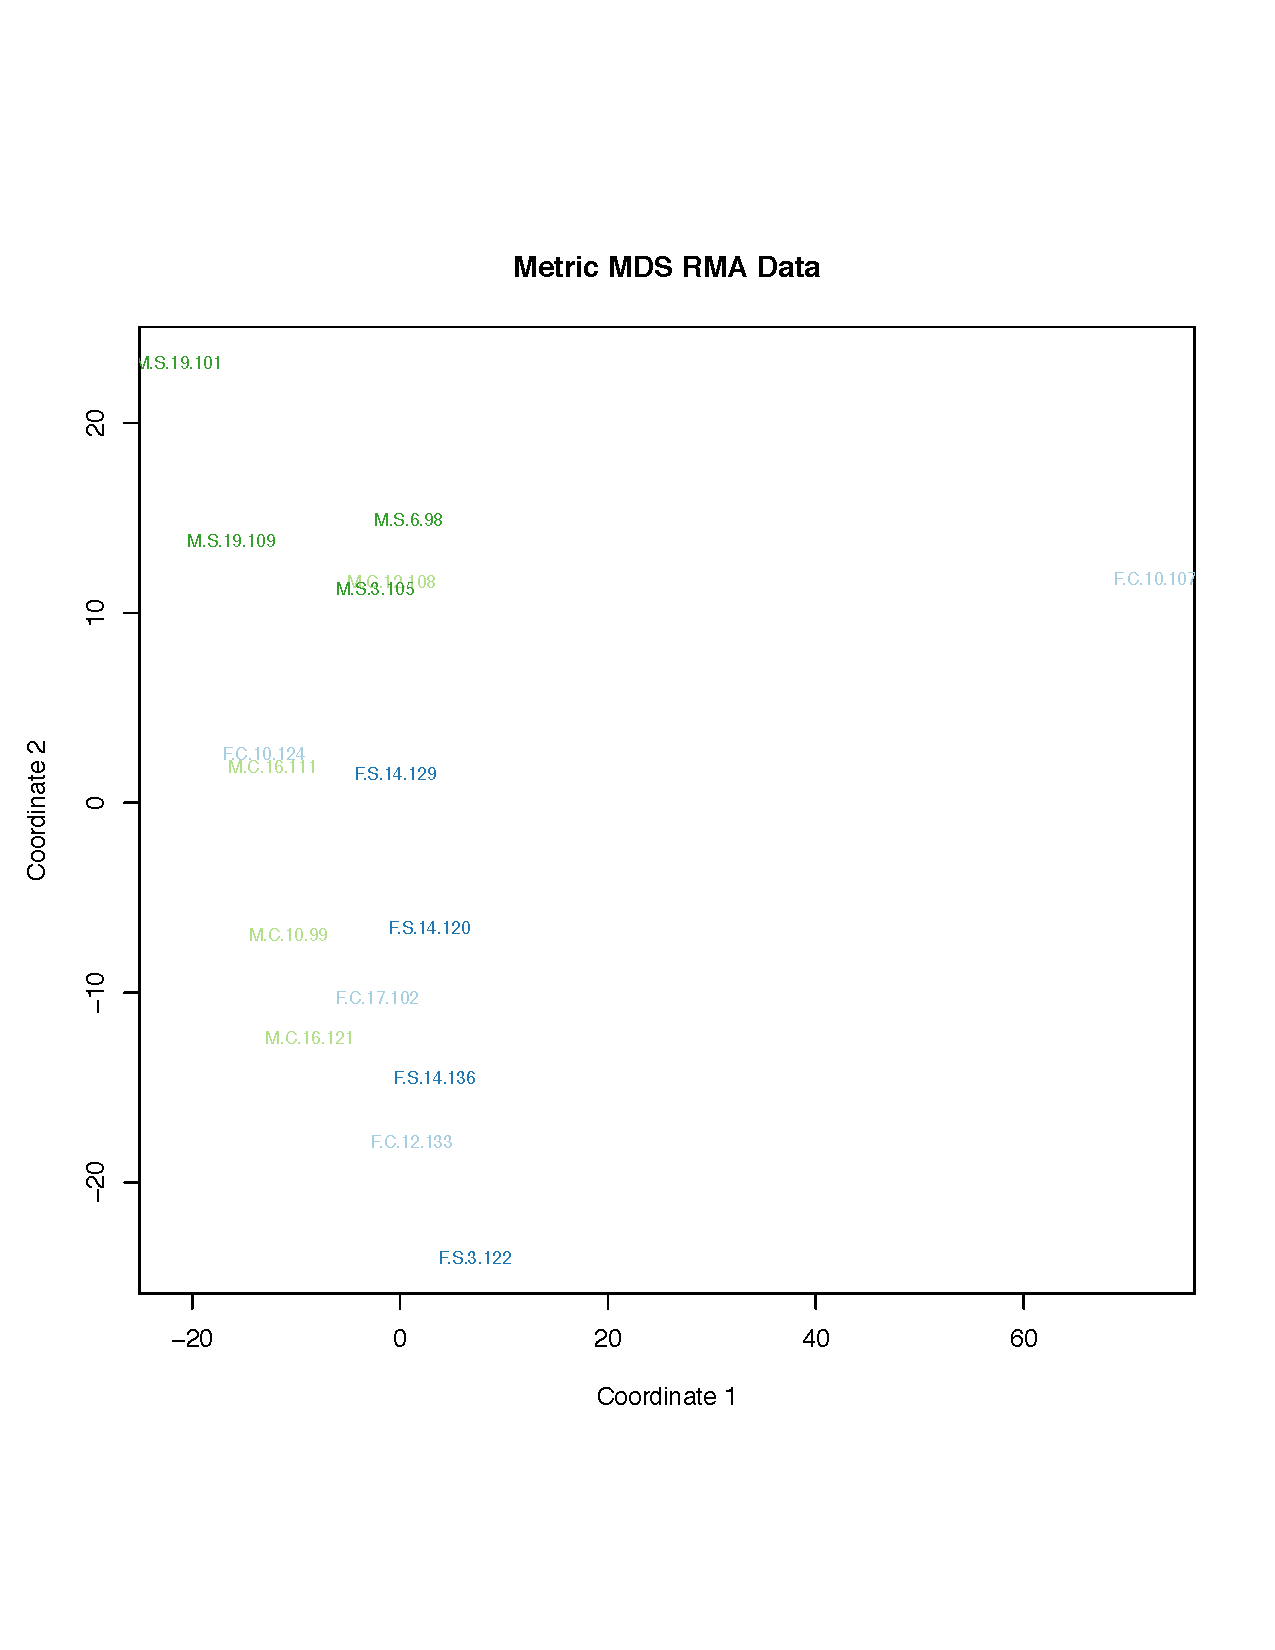
\includegraphics[scale=0.3]{figures/normMDS.pdf} 
\end{center}
\end{frame}

\section{Analysis Setup}
\begin{frame}
  \begin{itemize}
    \item \structure{Experiment\_Directory}
    \begin{itemize}
      \item \structure{Raw\_Data}
      \item \structure{Design\_Files}
      \item \structure{Figures}
      \item \structure{Tables}
      \item \structure{Data}
      \item Analysis.txt and/or Analysis.R
      \item targets.txt
    \end{itemize}
  \end{itemize}
\end{frame}

\begin{frame}
  \frametitle{targets.txt - an annotated data frame}
  An annotated data frame allows you to manage the samples for the experiment and includes at minimum sample names with associated raw data files. The framework however is flexible and allows for more information about samples to be included.\\


 \alert{See targets.txt file in example data} 
\end{frame}
  
\section{Public Repositories}
\begin{frame}
  \frametitle{Public Repositories for Microarrays Data}
  \begin{description}
    \item[GEO] \href{http://www.ncbi.nlm.nih.gov/geo/}{http://www.ncbi.nlm.nih.gov/geo/}
	\newline
    \item[ArrayExpress] \href{http://www.ebi.ac.uk/arrayexpress/}{http://www.ebi.ac.uk/arrayexpress/}
  \end{description}  
\end{frame}


%\frame{
%	\begin{description}
%	\item[Description]
%	A data driven approach for the computational and statistical understanding and expertise needed to solve bioinformatics problems that you will likely encounter in your research. 
%	\item[Goals]
%	Following this course the student will be capable of:
%	\begin{itemize} 
%		\item performing their own data analysis project, 
%		\item understanding the technical and statistical tools needed to conduct that analysis
%		\item have the computational ability to do the analysis
%		\item critically review and implement techniques and methods in publications.
%	\end{itemize}
%	\end{description}
%}
%
%\frame{

%\begin{frame}
%    \begin{columns}[c] % the "c" option specifies center vertical alignment
%    \column{.5\textwidth} % column designated by a command
%     Contents of the first column
%    \column{.5\textwidth}
%     Contents split \\ into two lines
%    \end{columns}
%\end{frame}
%
%\begin{frame}
%     \begin{columns}[t] % contents are top vertically aligned
%     \begin{column}[T]{5cm} % each column can also be its own environment
%     Contents of first column \\ split into two lines
%     \end{column}
%     \begin{column}[T]{5cm} % alternative top-align that's better for graphics
% Graphic would go here
%      \end{column}
%     \end{columns}
%\end{frame}
%
%\frame{
%   \begin{block}{This is a Block}
%      This is important information
%   \end{block}
% 
%   \begin{alertblock}{This is an Alert block}
%   This is an important alert
%   \end{alertblock}
% 
%   \begin{exampleblock}{This is an Example block}
%   This is an example 
%   \end{exampleblock}
%}

\end{document}
